\section{Methodology}
\label{sec:methodology}

Our study design follows directly from the threshold-plus-amplification hypothesis: we need an observational design that can isolate keyword tagging as the FAIR F1 operand, while controlling for the primary confounds --- dataset size, age, and platform era. Each design choice is a deliberate response to the problem structure.

\subsection{Dataset: OpenML Corpus}

We analyze the OpenML dataset corpus \citep{Vanschoren2014OpenML}, a cross-sectional snapshot of N=5,217 datasets with at least one registered ML task ($N\_tasks \geq 1$). OpenML is a publicly accessible ML experimentation platform where researchers register datasets, define ML tasks (target variable, task type), and execute experimental flows.

\textbf{Sample restriction ($N\_tasks \geq 1$):} We study conditional adoption intensity --- how tagging affects engagement among datasets that have been minimally engaged. Datasets with zero tasks are structurally different and would require a hurdle component for joint modeling; we defer this to future work.

\textbf{Key variables:}

\begin{table}[h]
\centering
\caption{Variable definitions for the OpenML corpus analysis.}
\label{tab:variables}
\begin{tabular}{lll}
\toprule
Variable & Role & Definition \\
\midrule
\texttt{N\_tasks} & DV & Count of distinct ML task registrations (integer $\geq 1$) \\
\texttt{has\_tags} & IV (P1) & Binary: 1 if dataset has $\geq$1 keyword tag, 0 otherwise \\
\texttt{log\_tag\_count\_p1} & IV (P2) & $\log(\text{tag\_count} + 1)$; restricted to \texttt{has\_tags=1} \\
\texttt{tag\_count\_cat} & IV (P3) & Categorical bins: 0, 1--2, 3--5, 6+ (reference: 0) \\
\texttt{log\_n\_instances} & Control & $\log(\text{number of instances})$ \\
\texttt{log\_n\_features} & Control & $\log(\text{number of features})$ \\
\texttt{age\_years} & Control & Dataset age in years \\
\texttt{age\_sq} & Control & \texttt{age\_years}$^2$ (quadratic age term) \\
\texttt{C(decade)} & Control & Decade-of-upload fixed effects \\
\bottomrule
\end{tabular}
\end{table}

\subsection{Model: Negative Binomial Type 2}

\textbf{Why NB-2 (not Poisson):} CT LR=7,356.36 ($\gg \chi^2(1)=3.84$ critical value) confirms strong overdispersion. Poisson regression would underestimate standard errors and inflate significance.

\textbf{Why binary \texttt{has\_tags} (not composite score):} A prior episode on the same corpus tested a composite metadata completeness score (0--5). That composite yielded IRR=1.076 under decade fixed effects, falling to IRR=1.014 ($p=0.19$). Binary \texttt{has\_tags} isolates the FAIR F1 signal without diluting it against non-F1 fields.

\textbf{Why decade fixed effects:} Platform era shifts created extreme decade-tag collinearity (Cram\'er's V=0.823). \texttt{C(decade)} controls for between-era confounding; we verify within-decade survival in the mechanism test.

\subsection{Four-Prediction Test Design}

\begin{table}[h]
\centering
\caption{Four-prediction test design with gate criteria.}
\label{tab:predictions}
\begin{tabular}{lllll}
\toprule
Prediction & Formula & Sample & Gate & Type \\
\midrule
P1 --- Binary Threshold & \texttt{N\_tasks $\sim$ has\_tags + controls + C(decade)} & N=5,217 & IRR$\geq$1.1, CI\_lower$\geq$1.1, $p<0.05$ & MUST\_WORK \\
Mechanism & P1 with vs.\ without \texttt{C(decade)} & N=5,217 & Post-FE IRR$\geq$1.1, $p<0.05$ & MUST\_WORK \\
P2 --- Log-Linear & \texttt{N\_tasks $\sim$ log\_tag\_count\_p1 + controls + C(decade)} & N=2,625 & CI\_lower$\geq$1.05, $p<0.05$ & SHOULD\_WORK \\
P3 --- Categorical & \texttt{N\_tasks $\sim$ C(tag\_count\_cat) + controls + C(decade)} & N=5,217 & Monotonic IRR, $\geq$2/3 adj.\ contrasts $p<0.0167$ & SHOULD\_WORK \\
\bottomrule
\end{tabular}
\end{table}

\begin{figure}[h]
\centering
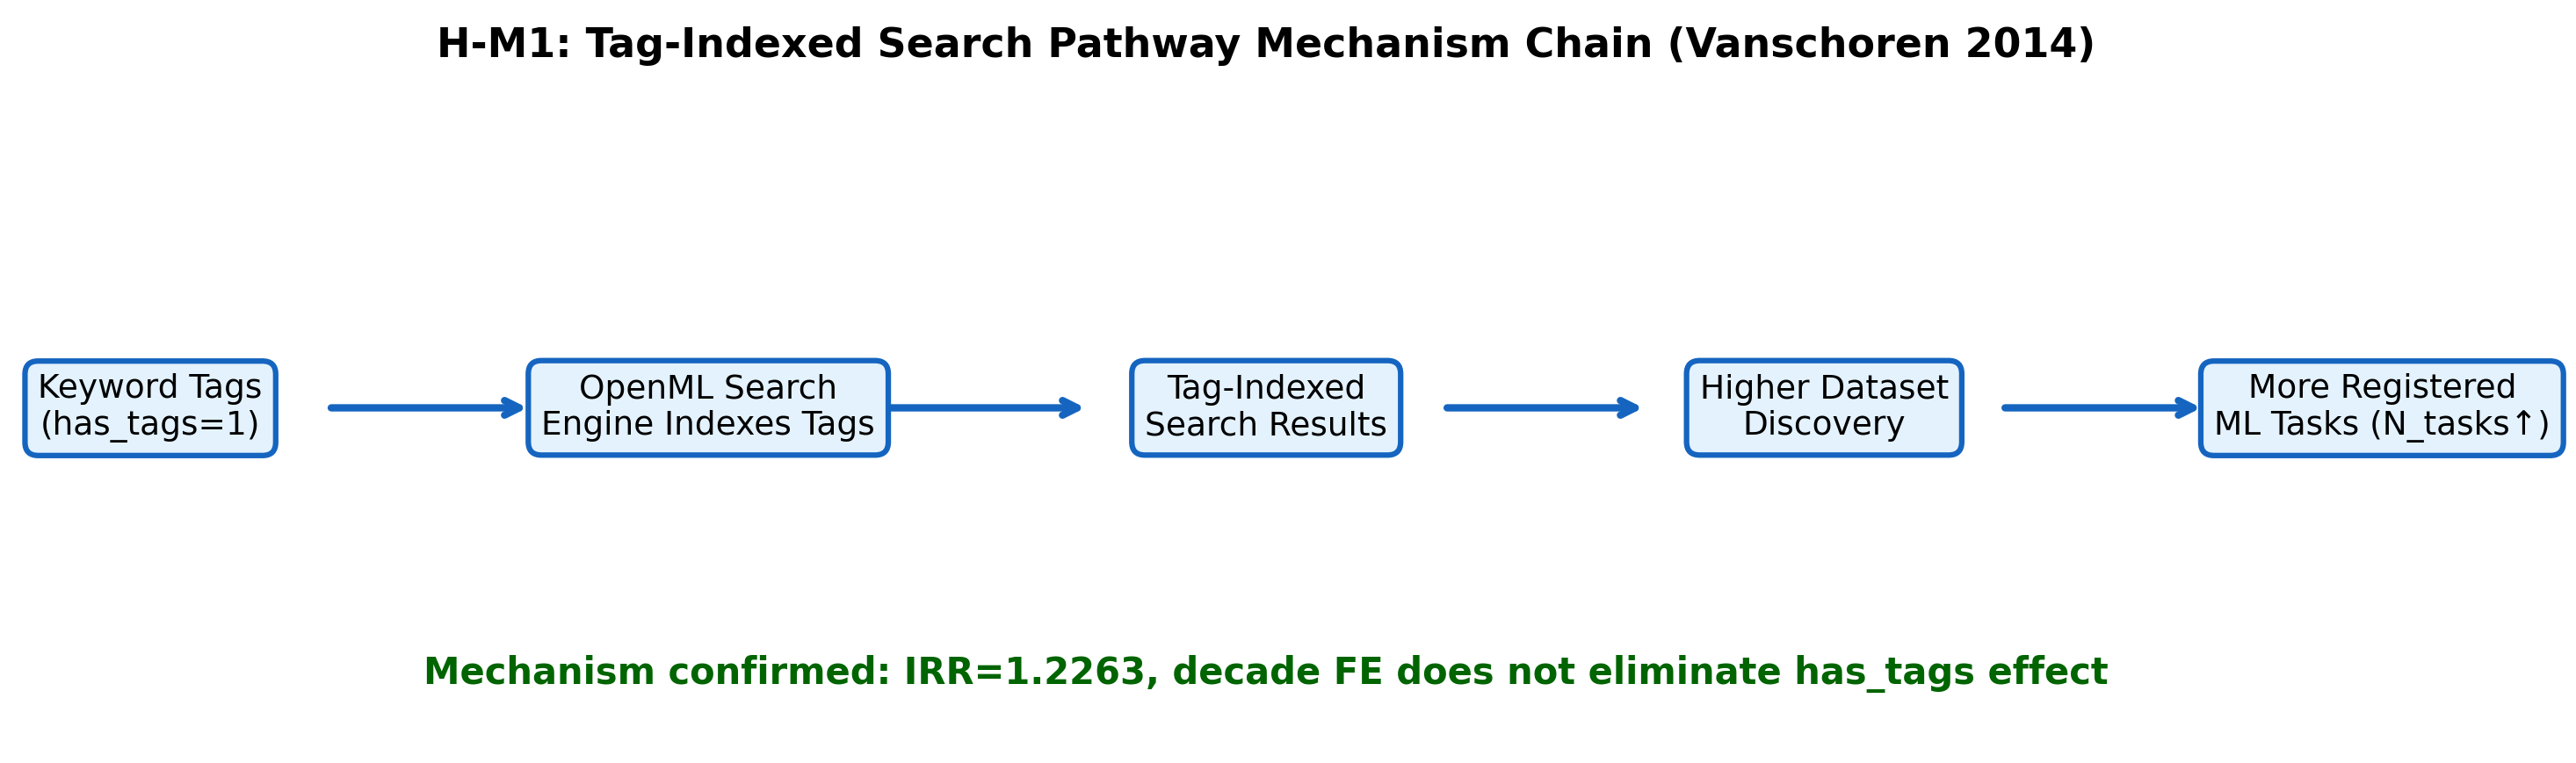
\includegraphics[width=0.7\linewidth]{figures/fig4_mechanism_flow.png}
\caption{FAIR F1 threshold-plus-amplification mechanism chain. Dataset keyword tags $\rightarrow$ search index membership $\rightarrow$ multiple search query pathways $\rightarrow$ researcher discovery events $\rightarrow$ ML task registration (\texttt{N\_tasks} $\uparrow$).}
\label{fig:mechanism_flow}
\end{figure}

\subsection{Implementation}

All models: \texttt{statsmodels.formula.api.negativebinomial}, \texttt{loglike\_method=`nb2'}, BFGS optimizer (\texttt{method=`bfgs'}, \texttt{maxiter=100}), convergent for all seven model variants. IRR $= \exp(\text{coefficient})$; CI $= \exp(\text{coefficient} \pm 1.96 \cdot \text{SE})$. Bonferroni correction for categorical contrasts: $\alpha=0.0167$ ($k=3$ contrasts). Across all four predictions, BFGS convergence was confirmed; results are reported in Section~\ref{sec:results} in causal-chain order (H-E1 $\rightarrow$ H-M1 $\rightarrow$ H-M2 $\rightarrow$ H-M3).
